\vspace{+20pt}
\part{Python Wrapper}
The Python wrapper is used to launch the pipeline analysis. 

\section{Start the pipeline}
The pipeline is launched in the \code{input} folder (see an example in \textbf{Figure \ref{fig:inputfolder}}). There are 3 key file types that \textbf{must} be present in each \code{Run} folder:
\begin{enumerate}
    \item the \textbf{FASTQ files} (in \code{fastq.gz} format) in their appropriate folder;
    \item the \textbf{file list} (in \code{csv} format) containing the sample IDs with their respective file names for R1 and R2;
    \item the \textbf{LIMS\_supp\_sample\_sheet} (in \code{csv} format) containing the information for each sample.
\end{enumerate}

Do not worry if more than one R1 and/or R2 file is present for one sample ID: as long as the file list is present, the program will handle them by itself.

Given these essential files, the \code{config.yaml} and the \code{sample\_info.csv} (needed for the rest of the pipeline) will be generated automatically in Run's folder.

To start the pipeline, the following command needs to be run in the \code{input} folder:

\begin{center}
    \lstinline[language=bash]{./StartPipeline.py -t [THREADS]}
\end{center}

\textcolor{Crimson}{\faExclamationCircle} \textbf{This command will run the pipeline, but you will need to stay connected to the terminal. }

If you want to run the pipeline and disconnect, you should run the command as follows:

\begin{center}
    \lstinline[language=bash]{nohup ./StartPipeline.py -t [THREADS] &}
\end{center}

The \code{-t} argument is optional and indicates the number of threads. If it is not specified, it will default to 39.\footnote{\textit{Note: bcl2fastq requires at least 16 threads.}} More information about multithreading can be found in \textbf{Section} \textbf{\ref{sec:multithreading}}.

\begin{figure}[H]
    \centering    
    \tikzset{every picture/.style={line width=0.75pt}} %set default line width to 0.75pt   
    \begin{tikzpicture}[x=0.75pt,y=0.75pt,yscale=-1,xscale=1]
        
        \draw (14,22) node [anchor=north west][inner sep=0.75pt]   [align=left] {\textcolor{Tan}{\faFolderOpen} input};
        \draw (24,42) node [anchor=north west][inner sep=0.75pt][align=left] {\textcolor{Tan}{\faFolder} \_\_pycache\_\_};
        \draw (25,62) node [anchor=north west][inner sep=0.75pt][align=left] {\textcolor{Tan}{\faFolder} .snakemake};
        \draw (26,82) node [anchor=north west][inner sep=0.75pt]   [align=left] {\textcolor{Tan}{\faFolderOpen} Run077};
        \draw (42,102) node [anchor=north west][inner sep=0.75pt]   [align=left] {\textcolor{Tan}{\faFolderOpen} FASTQ\_files};
        \draw (64,122) node [anchor=north west][inner sep=0.75pt]   [align=left] {\textcolor{SeaGreen}{\faFileCsv}  FASTQ\_file\_list.csv};
        \draw (64,142) node [anchor=north west][inner sep=0.75pt]   [align=left] {\textcolor{Sienna}{\faFileArchive}  Run...R1.fastq.gz};
        \draw (64,162) node [anchor=north west][inner sep=0.75pt]   [align=left] {\textcolor{Sienna}{\faFileArchive}  Run...R2.fastq.gz};
        \draw (70,182) node [anchor=north west][inner sep=0.75pt]    {$\vdots $};
        \draw (43,202) node [anchor=north west][inner sep=0.75pt]   [align=left] {\textcolor{SeaGreen}{\faFileCsv} LIMS\_supp\_sample\_sheet.csv};
        \draw (29,232) node [anchor=north west][inner sep=0.75pt]   [align=left] {\textcolor{Tan}{\faFolder} Run088};
        \draw (29,252) node [anchor=north west][inner sep=0.75pt] [align=left] {\textcolor{RoyalBlue}{\faPython} StartPipeline.py};
        \draw (29,272) node [anchor=north west][inner sep=0.75pt] [align=left] {\textcolor{RoyalBlue}{\faPython} Renaming.py};
    \end{tikzpicture}
    \caption{Example of the structure of the input folder.}
    \label{fig:inputfolder}
\end{figure}

\textcolor{Crimson}{\faExclamationCircle} \textbf{Note that the runs' folders must have the following name format: \texttt{Runxxx}}

\subsection{Getting the necessary files}
In the input folder, you will need to create the \texttt{Runxxx} folder and the \texttt{FASTQ\_files} subfolder.\\

To get the necessary files, you need to navigate to the run's directory:
\begin{center}
    \lstinline[language=bash]{cd /media/datasafe1b/ICGC_ARGO_CORE/runxxx_xxxxxx/FASTQ_files}
\end{center}

To copy the FASTQ files, run the following command:

\begin{lstlisting}[breaklines=true, language=bash]
for file in *.fastq.gz; do cp $PWD/$file ~/snakemake_watson/input/Runxxx/FASTQ_files/$file; done
\end{lstlisting}


You will then need to get the file list and the sample sheet. Do that as follows:
\begin{center}
    \lstinline[language=bash]{cp FASTQ_file_list.csv ~/snakemake_watson/input/Runxxx/FASTQ_files/}

    \lstinline[language=bash]{cp LIMS_supp_sample_sheet.csv ~/snakemake_watson/input/Runxxx/}
\end{center}

\subsection{Re-running the pipeline}
When you are running the pipeline on FASTQs that were already processed by Watson or Holmes, the file names will not change automatically (since their names will not correspond to the ones in the file list). They most probably will be found in the following format:

\begin{center}
    \texttt{08801\_AHHC3VBGXV\_Run088b01\_R1.fastq.gz}
\end{center}

You will need to rename them as follows:

\begin{center}
    \texttt{Run088b01\_R1.fastq.gz}
\end{center}

\section{Required files' format}
\subsection{LIMS\_supp\_sample\_sheet.csv}
This sheet should contain the following fields: LIMS\_ID, Sample\_ID, Project, SampleType, PreservationType, TumourType, Species, Gender, GermlineConsent, MatchNorm, AmountDNAused, LibConc, LibType, BaitsetID, SeqContID, TubeBarcode.

This sheet is needed to generate the following \code{sample\_info.csv} file:

\begin{table}[!ht]
    \centering
    \begin{tabular}{llll}
    \hline
        \textbf{LIMS\_ID} & \textbf{Gender} & \textbf{AmountDNAused} & \textbf{LibConc} \\ \hline
        Run077b09 & Male & 70 & 10.3 \\ 
        Run077b10 & Male & 70 & 13.8 \\ 
        Run077b11 & Male & 70 & 13.2 \\ 
        Run077b12 & Male & 70 & 11 \\ 
        Run077b13 & Male & 70 & 11.7 \\ 
        Run077b14 & Female & 70 & 12.2 \\ 
        Run077b15 & Female & 70 & 11.3 \\ 
        Run077b16 & Male & 70 & 11.2 \\ 
        Run010b10b & Female & 50 & 208 \\ 
        Run010b11b & Female & 50 & 193 \\ \hline
    \end{tabular}
\end{table}

If the \code{sample\_info.csv} does not have the fields from this example, check the \code{LIMS\_supp\_sample} \code{\_sheet.csv} file: most probably, the fields' names are not correct. To fix the issue, you can change the names of the corresponding fields. 

\subsection{FASTQ file list}
This list is required to handle file names different from the one required for the snakefile to work. It also concatenates files coming from the same sample to have just one file for R1 and one for R2. 

The format required for that file is the following:
\begin{table}[H]
    \centering
    \begin{tabular}{lllll}
    \hline
        \textbf{LIMS\_ID} & \textbf{Sample\_ID} & \textbf{Filename\_R1} & \textbf{Filename\_R2} & \textbf{...} \\ \hline
        Run077b09 & 07709 & 9\_S2\_L002\_R1\_001.fastq.gz & 9\_S2\_L002\_R2\_001.fastq.gz & ... \\ 
        Run077b09 & 07709 & 9\_S2\_L003\_R1\_001.fastq.gz & 9\_S2\_L003\_R2\_001.fastq.gz & ... \\ 
        $\vdots$ &&&& \\ \hline
    \end{tabular}
\end{table}

In particular, the headings \textbf{Sample\_ID}, \textbf{Filename\_R1} and \textbf{Filename\_R2} must be present (the order does not matter).

\section{Changing directories}
If you need to change directories for static files, snakefile, reference, output or input, you can change them in the script:
\begin{lstlisting}[breaklines=true, language=python, caption=Code section you will need to modify if you want to change directories.]
### --- CONFIG FILE AND SAMPLE INFO COMPILATION --- ###
# Static files
static_path = "/home/watson/snakemake_watson/static_files"
bin_path = "/home/watson/snakemake_watson/bin"
reference_path = "/home/watson/snakemake_watson/static_files/GRCh38.fa"
output_path = "/home/watson/snakemake_watson/output"

# Get runs
input_dir = "/home/watson/snakemake_watson/input"
\end{lstlisting}

\section{Multithreading}\label{sec:multithreading}
Parallel computing is handled directly by snakemake via slurm, but you can specify the number of threads to pass to the snakefile via the \code{-t} argument.

Since bcl2fastq requires at least 16 threads, the Python wrapper handles this as follows:
\begin{itemize}
    \item If the number of threads is not specified, it defaults to 39
    \item If the number of threads is specified, it checks if the number is at least 18 and the number of threads of the machine:
    \begin{itemize}
        \item If the number of threads of the machine is at least 18, the program sets the number of threads to 16 and throws a warning
        \item If the number of threads of the machine is less than 18, the program throws an error and exits
    \end{itemize}
\end{itemize}

\begin{lstlisting}[breaklines=true, language=python, caption=Code section you will need to change if you want to modify how you handle multithreading.]
# Handle threads number
if args.threads < 16:
    threads_count = psutil.cpu_count(logical=True)
    if threads_count < 18:
        sys.exit(f"ERROR: bcl2fastq requires at least 16 threads! \n You only have {threads_count} threads!")
    else:
        print(f"WARNING: bcl2fastq requires at least 16 threads! \n You have {threads_count} threads, number of threads is now set to 16.")
        T = 16
else:
    T = args.threads
\end{lstlisting}

\section{Output handling}
Every run will have its subfolder in the output directory:

\begin{figure}[H]
    \centering    
    \tikzset{every picture/.style={line width=0.75pt}} %set default line width to 0.75pt   
    \begin{tikzpicture}[x=0.75pt,y=0.75pt,yscale=-1,xscale=1]
        
        \draw (14,22) node [anchor=north west][inner sep=0.75pt]   [align=left] {\textcolor{Tan}{\faFolderOpen} output};
        \draw (24,42) node [anchor=north west][inner sep=0.75pt][align=left] {\textcolor{Tan}{\faFolderOpen} Run077};
        \draw (42,62) node [anchor=north west][inner sep=0.75pt][align=left] {\textcolor{Tan}{\faFolder} Run077b01};
        \draw (42,82) node [anchor=north west][inner sep=0.75pt]   [align=left] {\textcolor{Tan}{\faFolder} Run077b02};
        \draw (25,102) node [anchor=north west][inner sep=0.75pt][align=left] {\textcolor{Tan}{\faFolder} Run088};
    \end{tikzpicture}
    \caption{Example of the structure of the output folder.}
    \label{fig:outputfolder}
\end{figure}

The script will automatically remove all temporary files and the run folder in the input and rename the necessary files with the appropriate file name. 

\section{Checking if the pipeline was completed sucessfully}
To check if every rule was completed without errors you can use the \texttt{CheckCompleted.py} script as follows:
\begin{center}
    \lstinline[language=bash]{./CheckCompleted.py -i output/Runxxx/logs}
\end{center}

If the pipeline was completed successfully, you will see the following message:

\begin{lstlisting}
All samples were analyzed successufully.
\end{lstlisting}

Otherwise, you will see a list of the rules that failed and the samples that were not analyzed. An example would be:

\begin{lstlisting}
RuleName of sample SampleID was not completed.

Some samples failed. Check the logs for more information.
\end{lstlisting}